\section{Industrie- und Gewerbegrossspeicher}

\subsection{Batteriespeicher in Gewerbe}

\subsubsection{Motivation von gewerblichen Kunden für eine Solarbatterie}

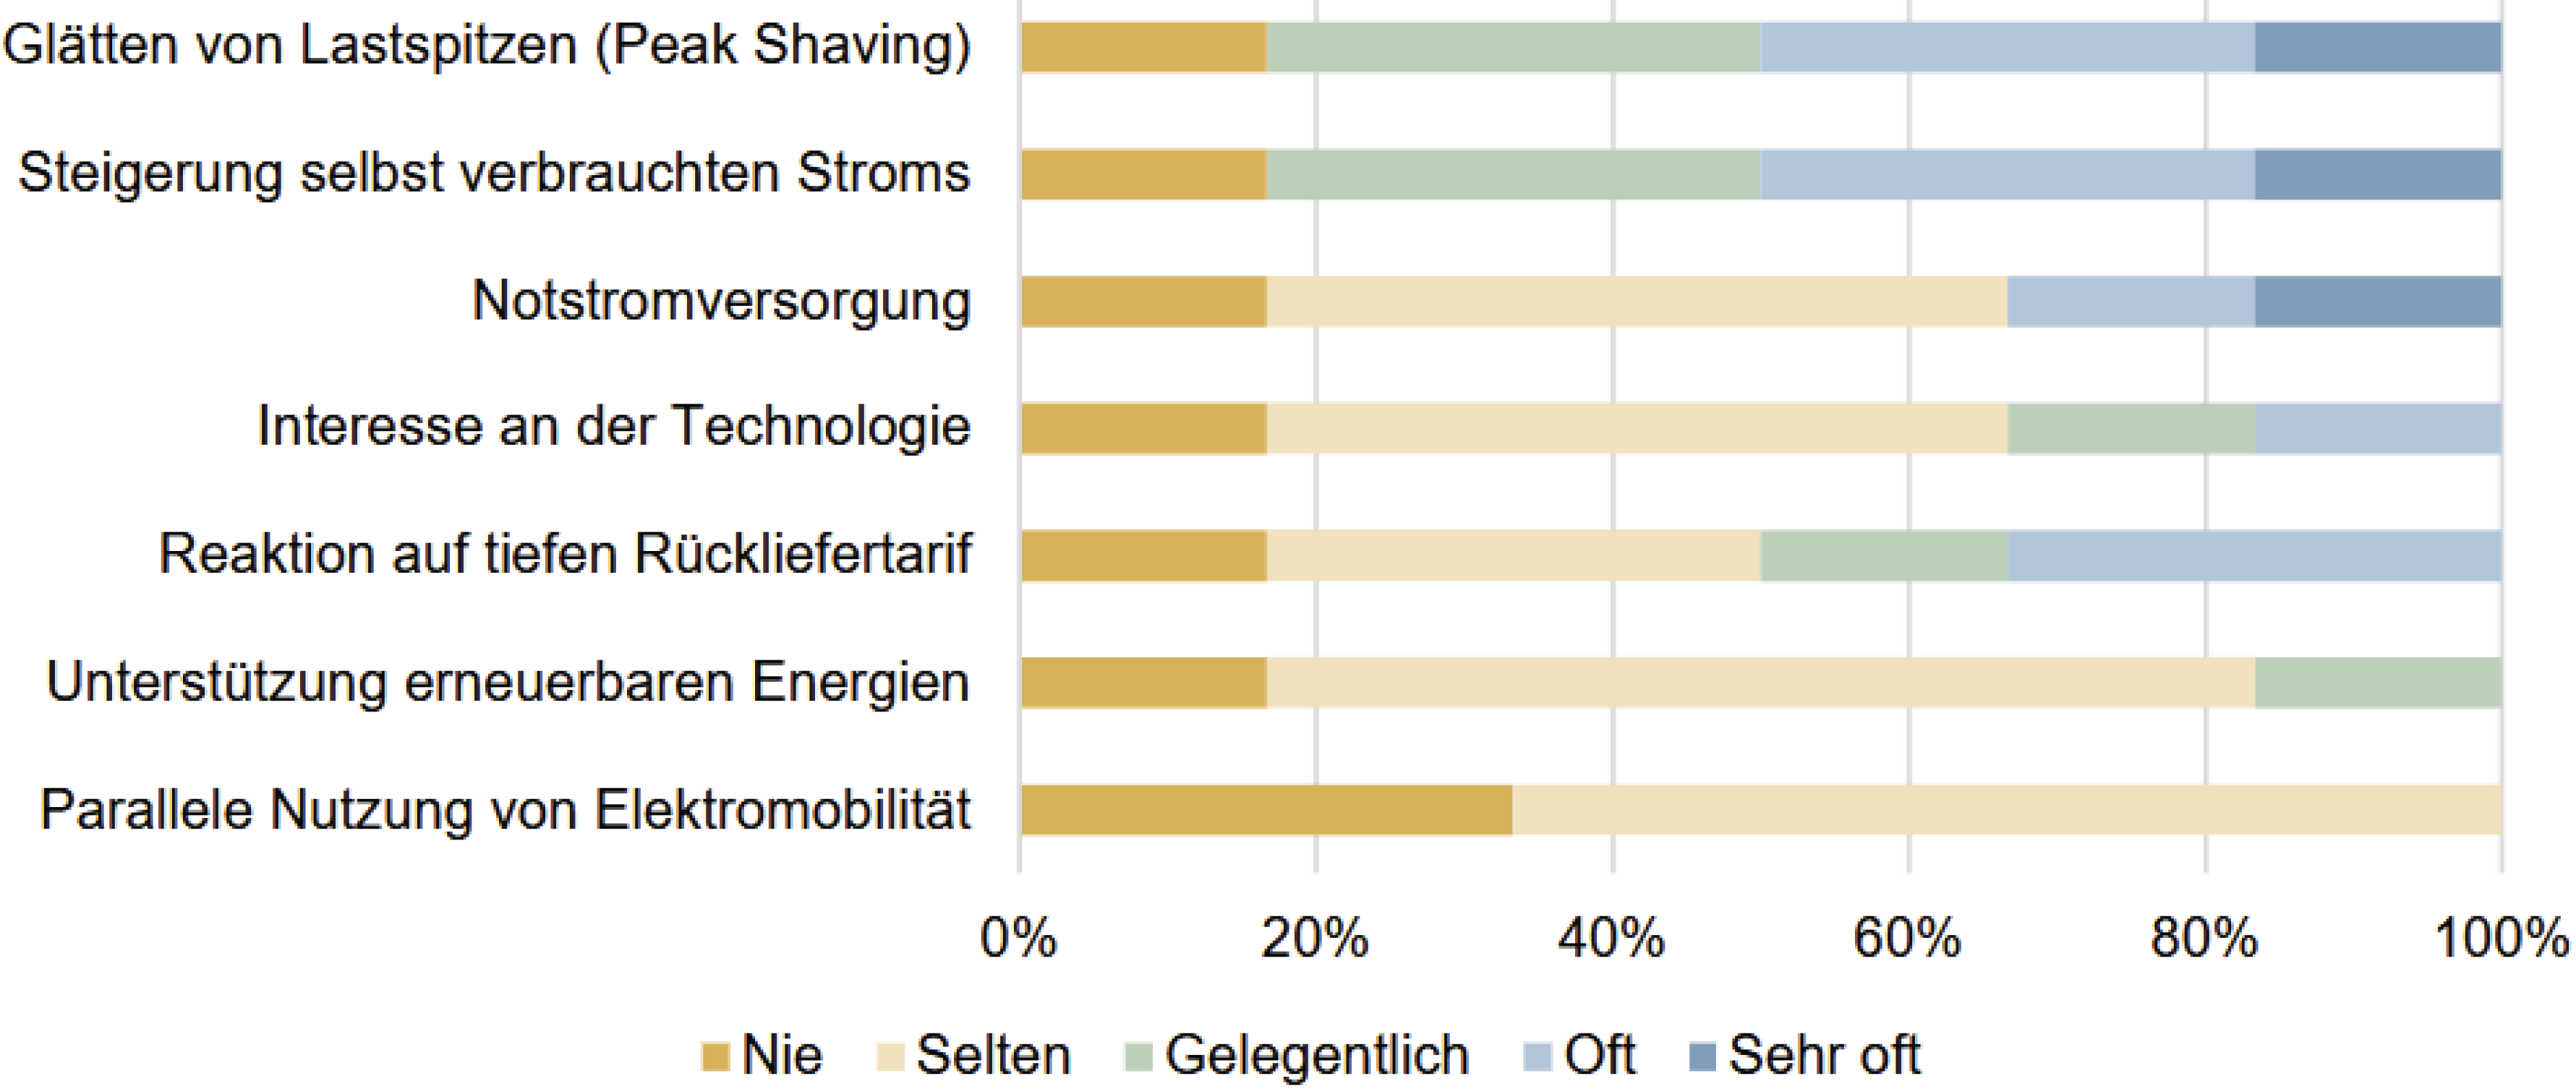
\includegraphics[width=0.98\columnwidth]{images/Batteriespeicher_im_Gewerbe.png}



\subsection{Quartier- und Grossspeicher}

\begin{itemize}
  \item \textbf{Betrieb häufig durch Netzbetreiber}
  
  \item \textbf{Motivation / Möglichkeiten}
  \begin{itemize}
    \item Vermarktung "Eigenverbrauch" an Kunden
    \item Vermeidung von Netzengpässen (Verschiebung von Last- und Einspeisespitzen)
    \item Bereitstellung von Regelleistung (mind. 1 MW für Primärregelleistung, mind. 5 MW für Sekundärregelleistung, auch mit mehreren Speichern möglich)
    \item Für Verteilnetzbetreiber: Reduzierung der Kosten gegenüber vorgelagertem Netz (Leistungspreis) durch Peak-Shaving
    \item Flexibilität bei Energiebeschaffung am Strommarkt (Termin-, Spot-, Intradaymarkt)
    \item Fahrplanmanagement, Bilanzausgleich zur Vermeidung von Strafzahlungen
    \item Unterstützung Spannungshaltung durch Blindleistungseinspeisung (durch Wechselrichter)
    \item Dynamische Anpassung bei Kurzschlusssituationen (Kompensierung von Leistungstransienten und Vermeidung von Überstromsituationen z.\,B. bei Schaltvorgängen)
  \end{itemize}
\end{itemize}


\subsubsection{Beispiel EKZ}



\subsubsection{Beispiel EWJR}




\subsection{Batteriespeicher in Industrie und Gewerbe}
\begin{itemize}
    \item Motivation: Reduktion von Energiekosten, Netzstabilisierung
    \item Multi-Use Konzepte: Eigenverbrauch, Peak-Shaving, Vermarktung von Flexibilität
\end{itemize}

\subsection{Quartier- und Grossspeicher}
\begin{itemize}
    \item Anwendung durch Netzbetreiber: Netzengpässe vermeiden, Regelleistung bereitstellen
    \item Unterstützung von Bilanzkreisausgleich, Fahrplanmanagement
    \item Beispiele:
    \begin{itemize}
        \item EKZ: 18 MW Leistung, 7.5 MWh Kapazität
        \item EWJR: Erweiterung auf 6 MW / 6 MWh
    \end{itemize}
\end{itemize}

\subsection{Regelleistung}
\begin{enumerate}
    \item Primärregelleistung (30 Sekunden)
    \item Sekundärregelleistung (5 Minuten)
    \item Tertiärregelleistung (15 Minuten)
\end{enumerate}


























